\section{\textit{WBS}}

 \begin{figure}[!ht]
	\centering
		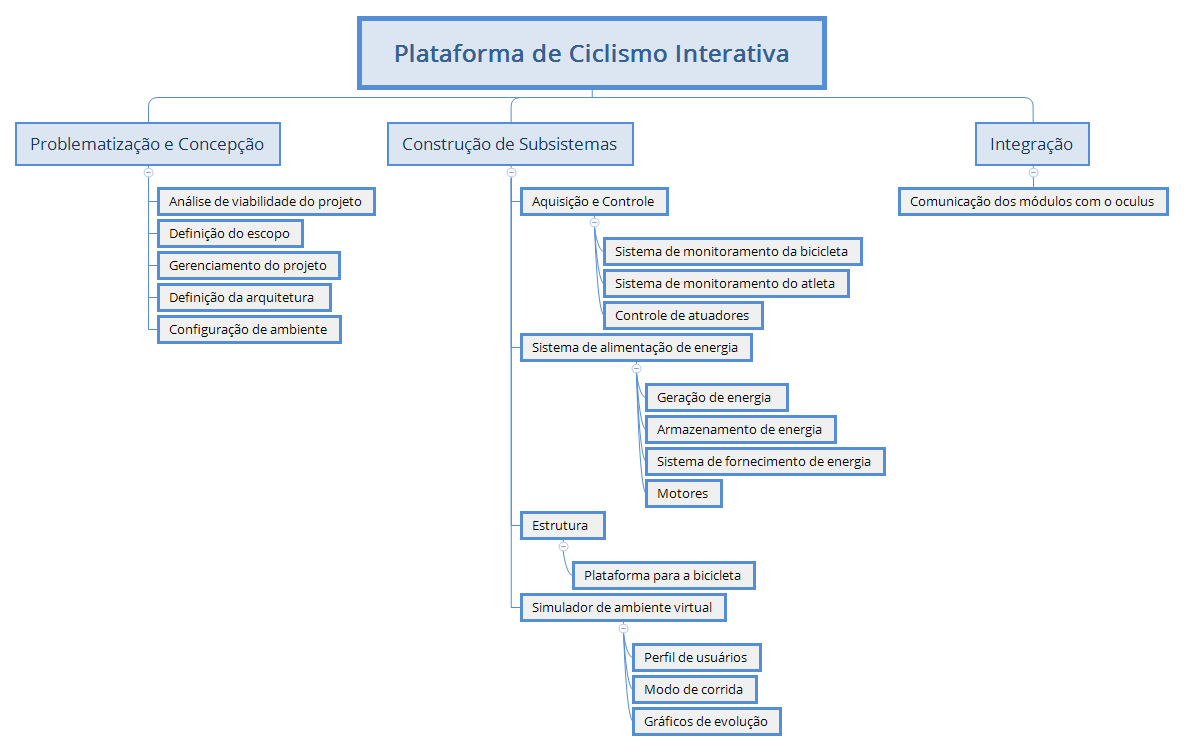
\includegraphics[scale=0.4]{figuras/eap}
	\caption{Estrutua Analítica do Projeto.}
\end{figure} 

\section{Lista É/Não É}

\begin{itemize}
\item O jogo é um simulador de um ambiente de corrida de bicicleta gamificado que utiliza informações reais do usuário.
\item O jogo não é uma a simulação de um ambiente para a exploração do usuário.
\item O jogo mostra as medidas do desempenho do usuário comparando-as com resultados anteriores. O design gráfico do jogo não é realista.            

\item É um produto que possui um sistema de conversão de energia.
\item Não é um produto que possui um sistema de alimentação de energia integrado a rede elétrica convencional.
\item É um produto em que a alimentação principal ocorre por meio de bateria(s).
\item É um produto que possui um sistema de alimentação parcialmente autônomo.
\item É um produto que possui um sistema de alimentação com referências sustentáveis.

\item É uma estrutura adaptável.
\item Não é uma estrutura simples de treino de ciclismo.
\item É uma estrutura modular.
\item Não é uma bicicleta ergométrica.

\item É um produto com aquisição de dados através de sensores
\item É um produto modularizado com modulos comunicantes
\item Não é um produto com comunicação totalmente sem fio
\item É um produto que faz uso de um protocólo de comunicação


\end{itemize}


